\documentclass{if-beamer}
\usepackage{animate}
\usepackage{pythonhighlight}

% --------------------------------------------------- %
%                  Presentation info	              %
% --------------------------------------------------- %
\title[CS528 Final Presentation]{Gas Molecules Random Walk}
\subtitle{CS528 Final Presentation}
\author{Andrew Dunn}
\institute[CWU CS]{
  Department of Computer Science\\
  Central Washington University
}
\date{\today}

%\logo{
%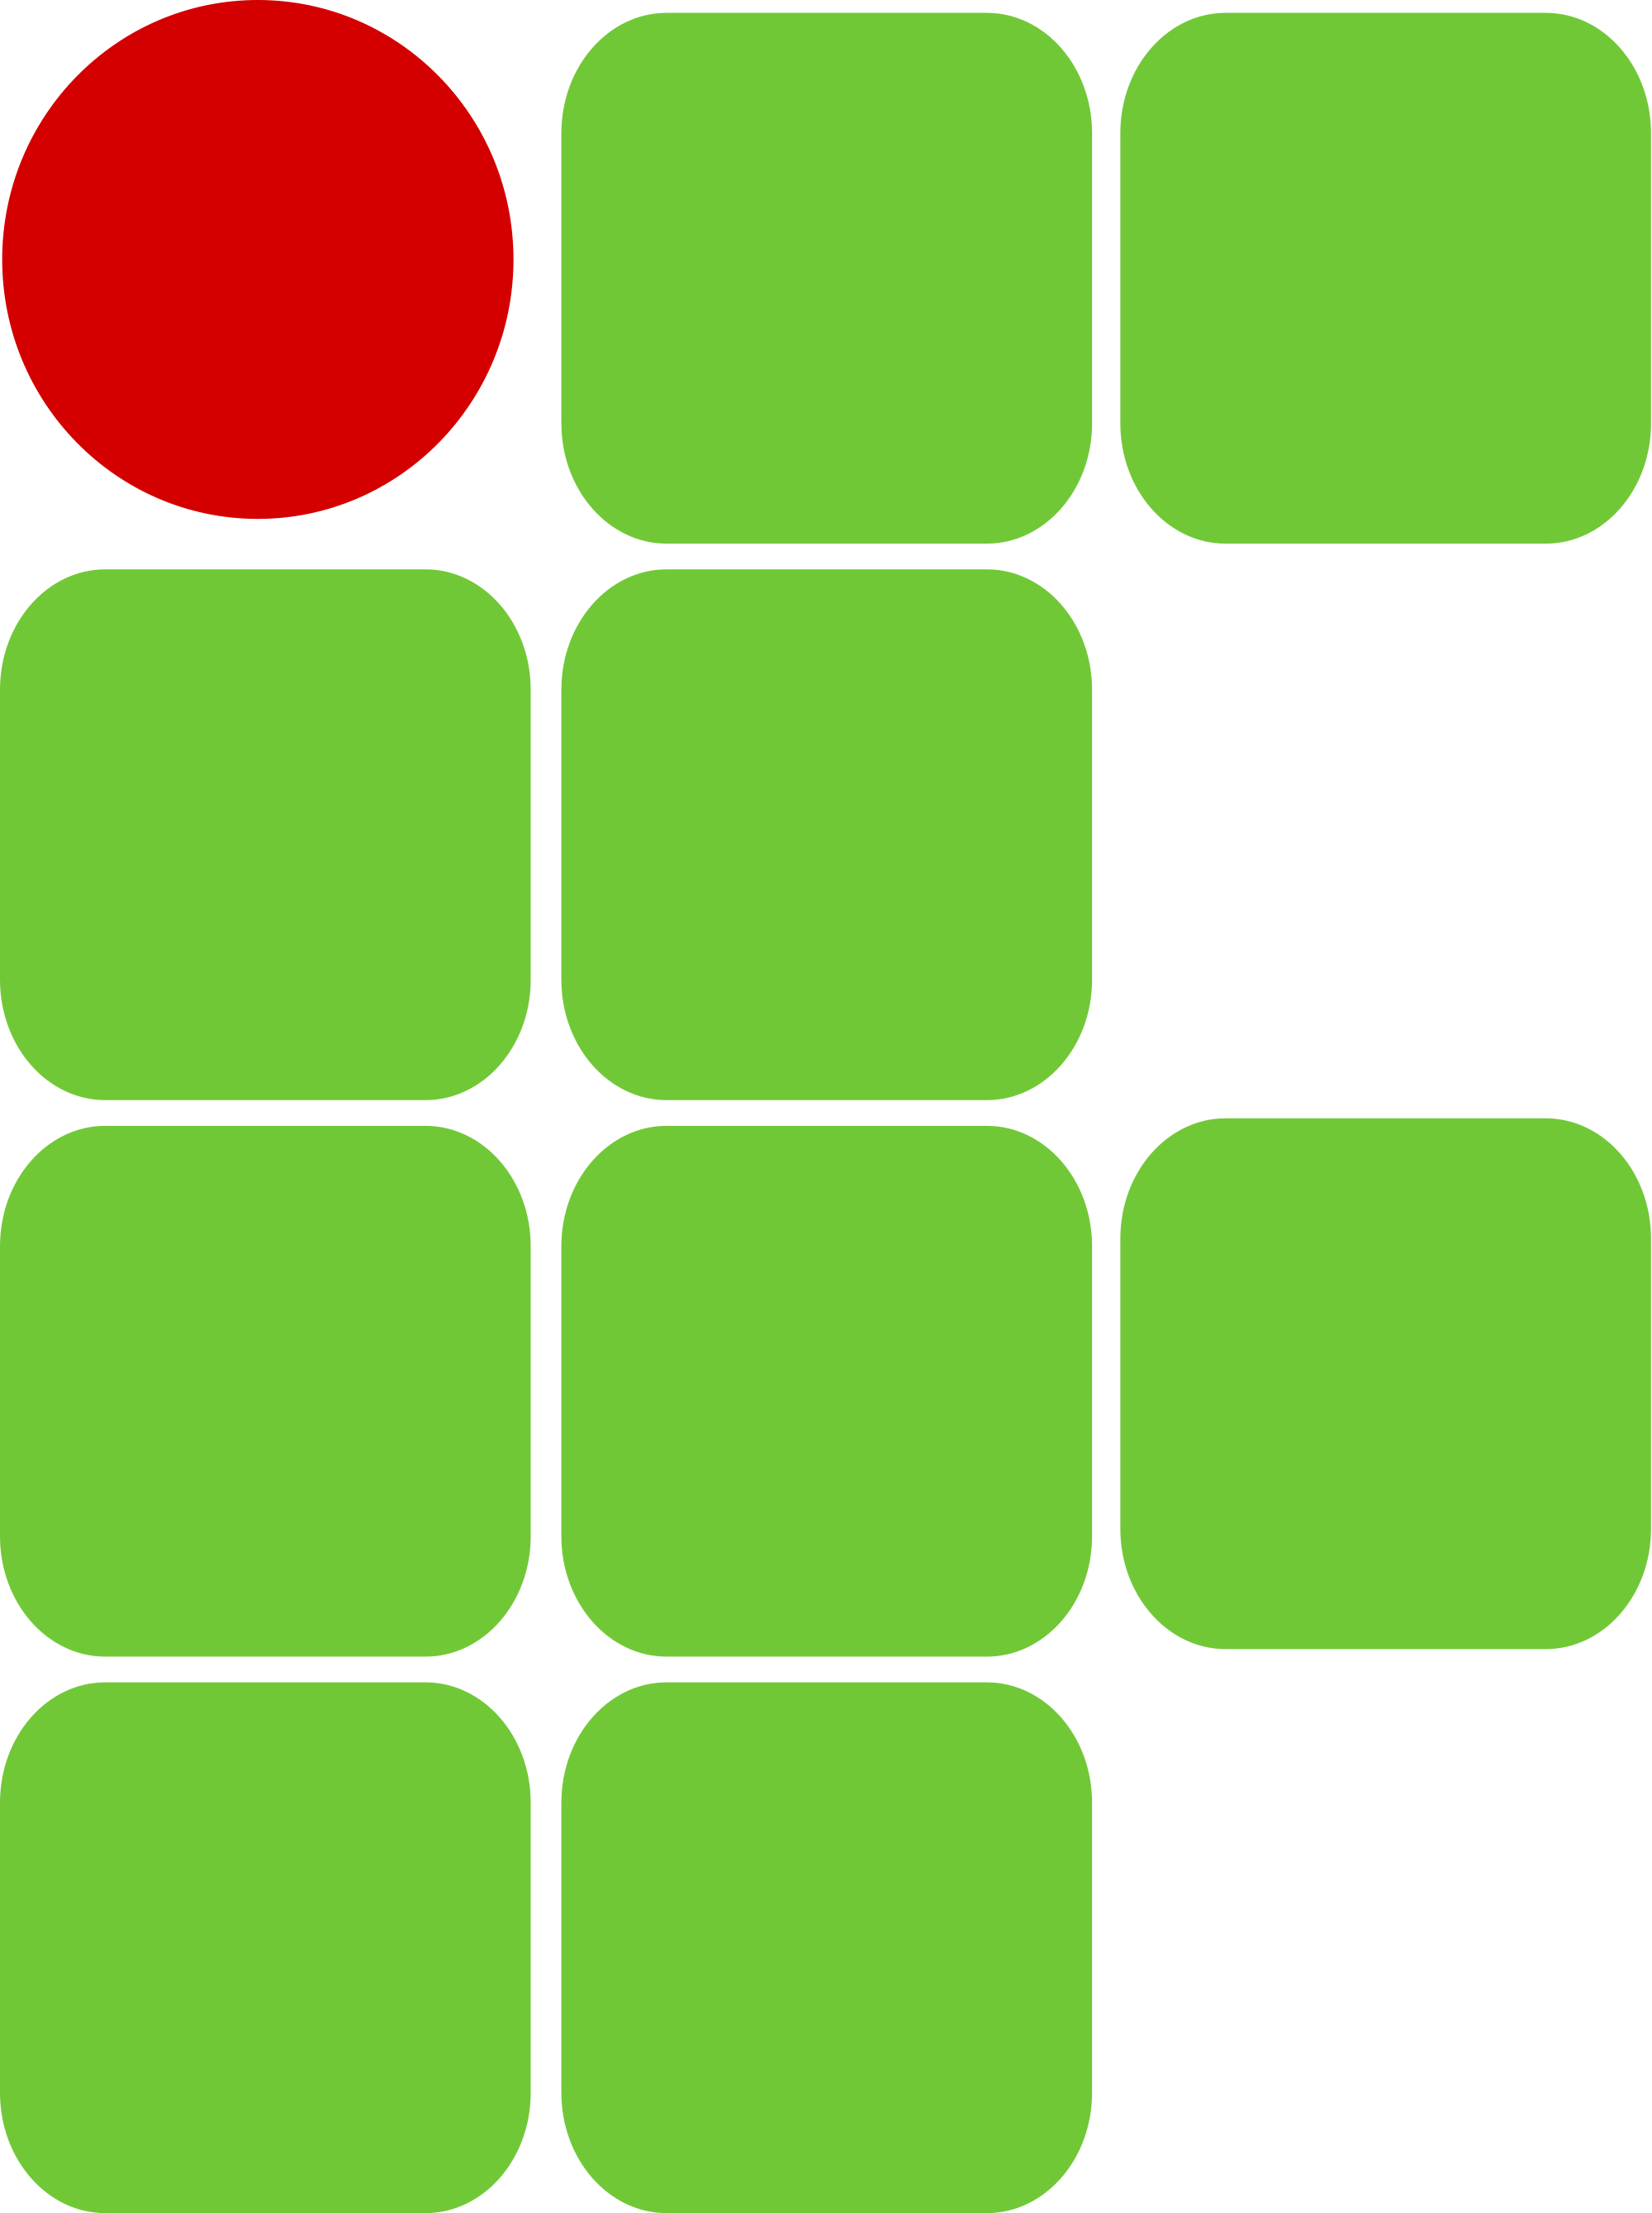
\includegraphics[scale=0.0065]{ifes-logo.png}
%}
\subject{CS528 Final Presentation} % metadata

\graphicspath{{figures/}}
% --------------------------------------------------- %
%                    Title + Schedule                 %
% --------------------------------------------------- %

\begin{document}

\begin{frame}
  \titlepage
\end{frame}

\begin{frame}{Outline}
  \tableofcontents
\end{frame}

% --------------------------------------------------- %
%                      Presentation                   %
% --------------------------------------------------- %
\section{Problem Description and Tools}

\begin{frame}{Problem Description}
  \begin{itemize}
  	\item Gas molecule simulation in closed space
  	\item 10,000 molecules randomly generated
  	\item Molecules start in partitioned sub-space
  	\item Random walk moves each molecule in random direction
  \end{itemize}
\end{frame}

% ==============================

\begin{frame}{Tools}
  \begin{itemize}
  	\item Python
  	\item Numpy
    \item Matplotlib/animation package
  \end{itemize}
\end{frame}

\begin{frame}{Random Walk Method} 
	
	\begin{figure}
		\centering
		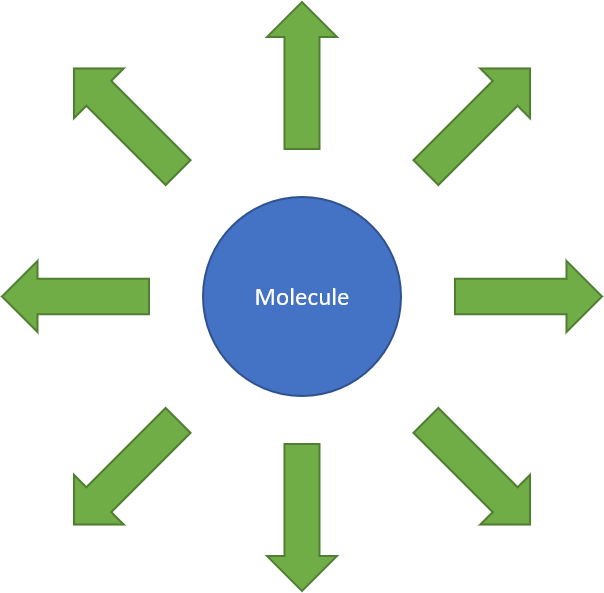
\includegraphics[scale=0.6]{molecule.png}
		\caption{Single Molecule Random Walk}
	\end{figure}
	
\end{frame}

\section{The Code}

\begin{frame}[fragile]{Random Walk Procedure}
\begin{python}
NUM_MOLECULES = 10000
RANDOM_WALK_DIST = 0.01

# ...

for i in range(NUM_MOLECULES):
    randAngle = np.random.uniform(np.pi * -1, np.pi)
    randVector = np.array([np.cos(randAngle), np.sin(randAngle)])
    randVector = randVector * RANDOM_WALK_DIST
    molX[i] = max(min(molX[i] + randVector[0], 1), 0)
    molY[i] = max(min(molY[i] + randVector[1], 1), 0)
\end{python}
\end{frame}

\begin{frame}[fragile]{Animated Plot Procedure}
	\begin{python}
class animatedScatter:
    def __init__(self, molXHist, molYHist):
    self.molXHist = molXHist
        self.molYHist = molYHist
        self.fig = plt.figure()
        self.fig.set_size_inches(PLOT_WIDTH, PLOT_HEIGHT)
        self.ax = plt.axes(xlim=(0, 1), ylim=(0, 1))
        self.itertext = self.ax.text(0.70, 0.9,  '', bbox=dict(facecolor='white', alpha=0.2), transform=self.ax.transAxes)
        print("Creating animation ... Please wait ...")
        self.ani = FuncAnimation(self.fig, self.update, frames=len(molXHist), interval=30, 
                init_func=self.setup, blit=True)
        print("Saving gif ... Please wait ...")
        self.ani.save('final_animated.gif', writer='imagemagick')
    def setup(self):
        self.scatter = self.ax.scatter([], [], color = "green")
        return self.scatter,
    def update(self, i):
        self.itertext.set_text('iteration = %d' % (i * ANIM_FRAMES_TIMESTEP))
        self.scatter.remove()
        self.scatter = self.ax.scatter(self.molXHist[i], self.molYHist[i], color = "green", alpha=0.2)
        return self.scatter,
	\end{python}
\end{frame}

\section{Results}

\begin{frame}{Execution Times}
	\begin{columns}
		\begin{column}{0.8\textwidth}
			\begin{tcolorbox}[tableblue,tabularx={X||Y}, boxrule=0.5pt, title=Execution Times]
				Number of Molecules & Time (sec) \\\hline\hline
				100    & 7.5    \\\hline
				1,000  & 74.51  \\\hline
				10,000 & 725.54 \\
			\end{tcolorbox}
		\end{column}
	\end{columns}
\end{frame}

\begin{frame}{Example 1 - 100 molecules and slow animation}
	\begin{center}
		\animategraphics[loop,controls,width=\linewidth]{20}{slow-anim/final_animated_slow-}{0}{200}
	\end{center}
\end{frame}

\begin{frame}{Example 2 - 1,000 molecules and fast animation}
	\begin{center}
		\animategraphics[loop,controls,width=\linewidth]{30}{1000-anim/1000_animated-}{0}{400}
	\end{center}
\end{frame}

\begin{frame}{Example 3 - 10,000 molecules and fast animation}
	\begin{center}
		\animategraphics[loop,controls,width=\linewidth]{30}{final-anim/final_animated-}{0}{400}
	\end{center}
\end{frame}

\section{Conclusion}

\begin{frame}{Conclusion}
	\begin{itemize}
		\item The molecule project was interesting
		\item CS528 has been a great learning experience
		\item LaTeX and Beamer are really useful
		\item Thank you Dr. Andonie for the quarter!
	\end{itemize}
\end{frame}

\begin{frame}{Questions?}
	\begin{center}
		\alert{Any Questions?}
	\end{center}
\end{frame}

\end{document}
